\section{Description et justification de la structure fonctionnelle}

\subsubsection*{Objectifs}

Cette section présente l'organisation fonctionnelle du système et la répartition des rôles entre les différents sous-ensembles. Chaque bloc (réception de trame, mémoire FIFO, registre d'état, interface microprocesseur) est décrit dans sa fonction et ses interactions avec les autres.  
L'objectif est de montrer comment les fonctionnalités définies lors de la spécification sont structurées logiquement pour répondre au cahier des charges, tout en restant indépendantes de toute technologie d'implémentation.

\begin{figure}[H]
    \centering
    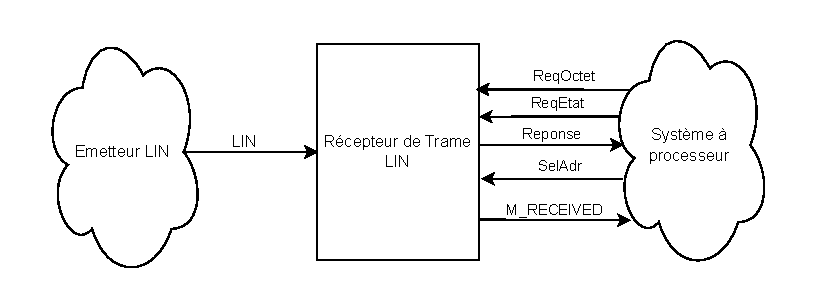
\includegraphics[width=0.8\linewidth]{images/inter/Structure_Fonc_Circuit.pdf}
    \caption{Représentation fonctionnelle des échanges entre l'émetteur LIN et le système à processeur}
    \label{fig:structure_fonc}
\end{figure}

À ce stade, le système est structuré autour de deux blocs principaux :  
l'interface microprocesseur et la réception des trames LIN.  
Ces deux blocs communiquent via un bloc d'échange chargé d'assurer la cohérence des transferts d'informations et la coordination entre les différents registres internes.

\begin{figure}[H]
    \centering
    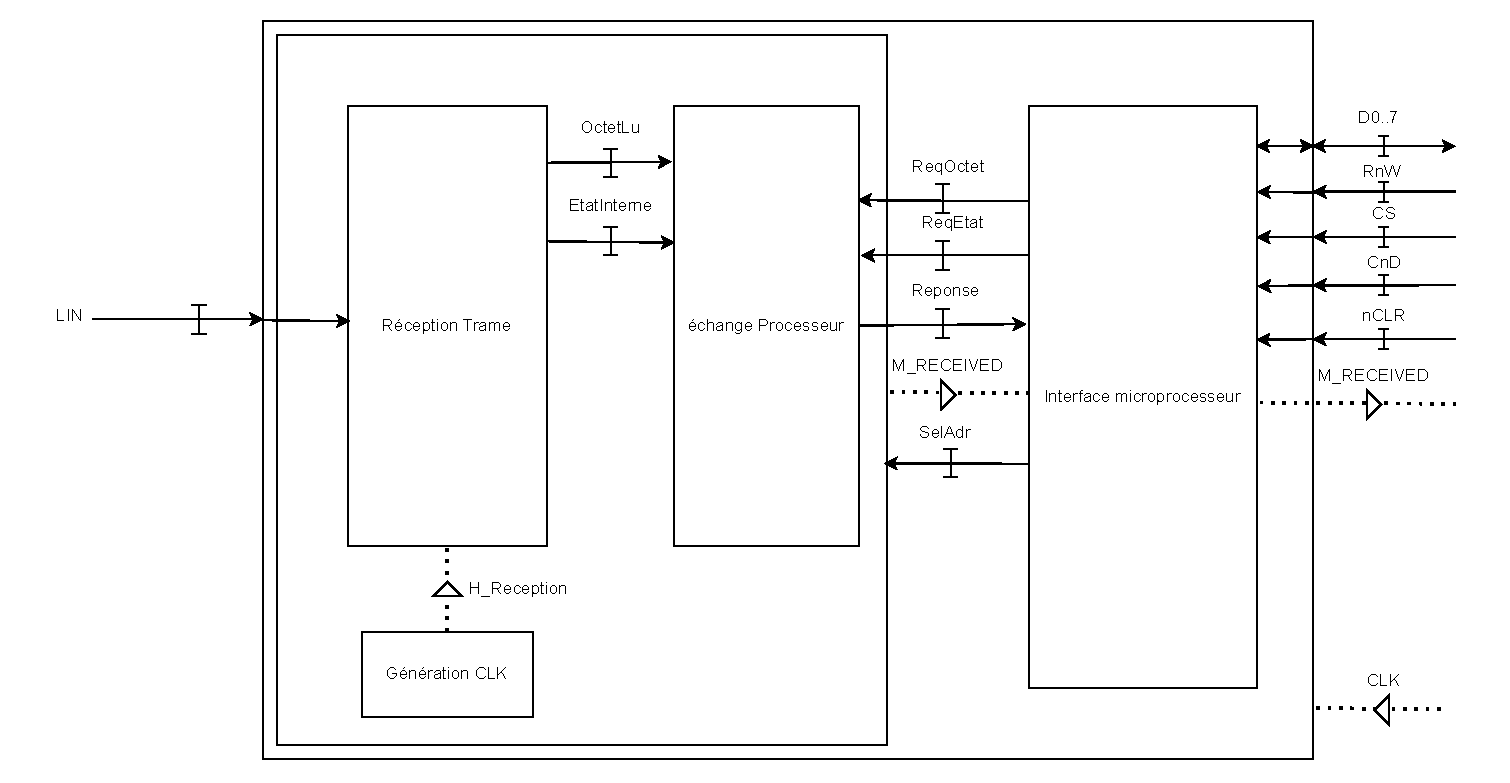
\includegraphics[width=0.8\linewidth]{images/inter/Schema_base_circuit.pdf}
    \caption{Structure fonctionnelle initiale du circuit après introduction des interfaces}
    \label{fig:schema_base_circuit}
\end{figure}

Le comportement général peut être représenté par un automate de communication illustrant les échanges avec le processeur :

\begin{figure}[H]
    \centering
    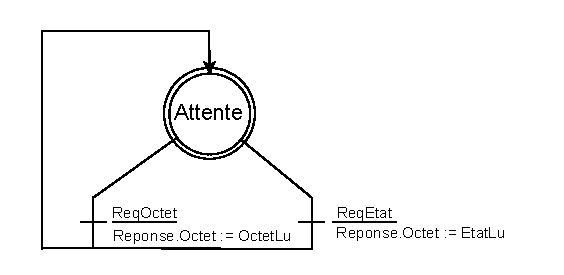
\includegraphics[width=0.8\linewidth]{images/inter/Echange_Processeur.pdf}
    \caption{Échanges fonctionnels entre le système et le processeur}
    \label{fig:echange_processeur}
\end{figure}

Lors de la phase d’analyse, il est apparu que le bloc d’échange microprocesseur pouvait être intégré directement à l’interface microprocesseur.  
Cette simplification permet de réduire le nombre de signaux intermédiaires et d’améliorer la clarté fonctionnelle du système.

\begin{figure}[H]
    \centering
    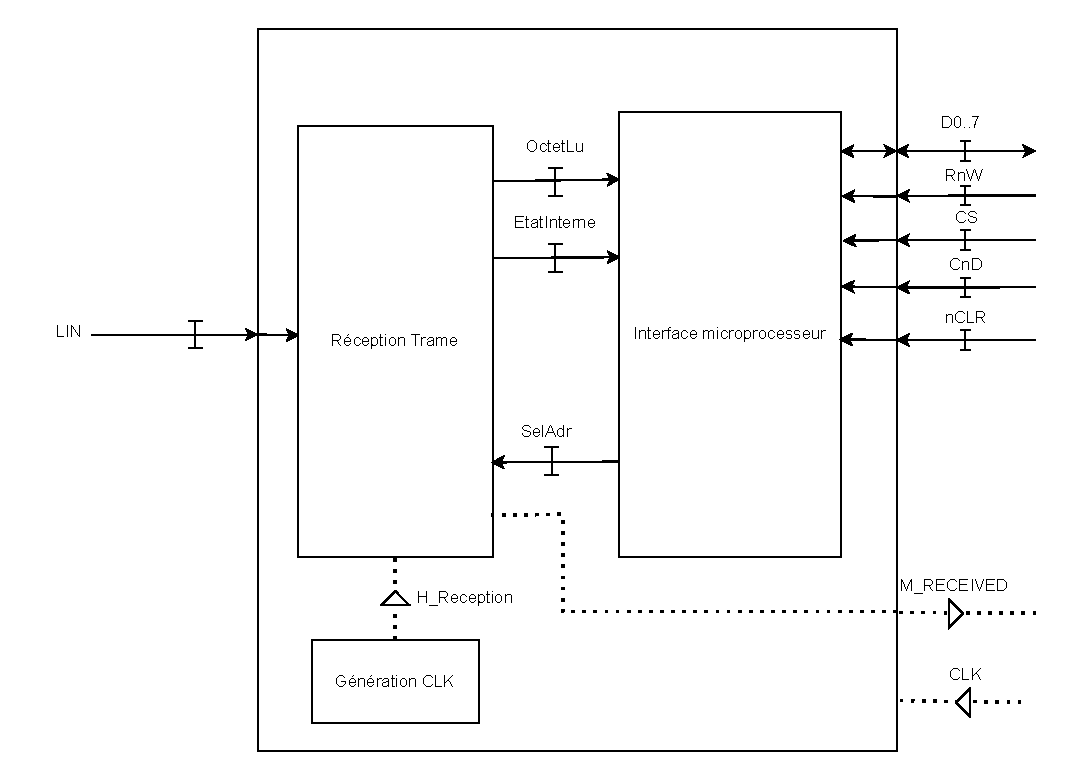
\includegraphics[width=0.8\linewidth]{images/inter/Schema_avance_circuit.pdf}
    \caption{Architecture fonctionnelle optimisée du système de réception de trame LIN}
    \label{fig:schema_avance_circuit}
\end{figure}

Enfin, deux registres internes ont été ajoutés :  
\begin{itemize}
    \item un registre de stockage des données de trame (FIFO) ;
    \item un registre d'état interne (ETAT), contenant les informations de suivi et d’erreur.
\end{itemize}

\begin{figure}[H]
    \centering
    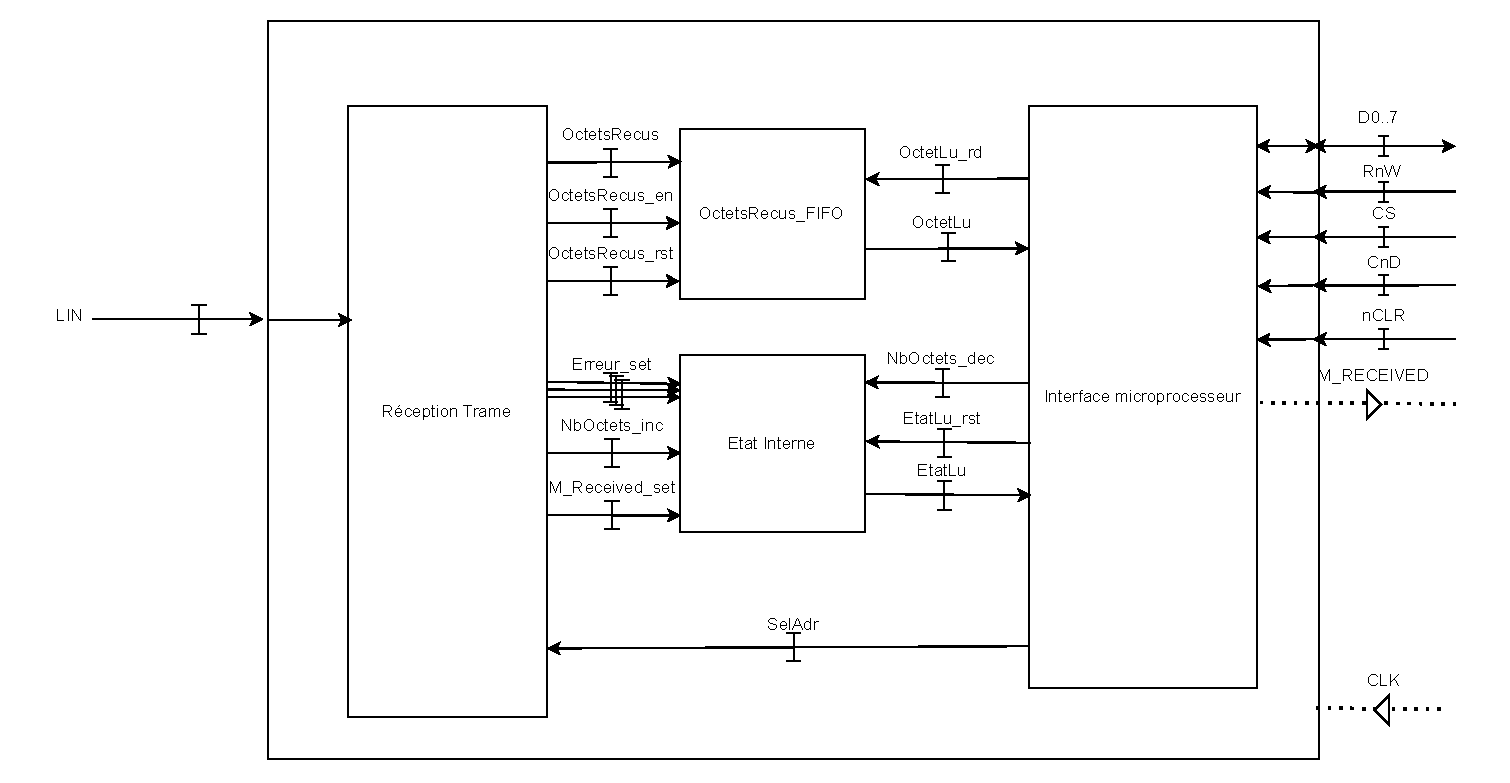
\includegraphics[width=0.8\linewidth]{images/inter/Schema_Final.pdf}
    \caption{Description fonctionnelle finale du circuit complet}
    \label{fig:schema_final}
\end{figure}

Le schéma global ci-dessus illustre les interactions fonctionnelles entre les différents blocs du système. Les échanges sont exprimés en termes de flux d’informations (données, ordres, signaux de contrôle), sans référence à la nature physique ou logique de ces signaux.

\subsubsection*{Bloc FIFO}

\begin{center}
\renewcommand{\arraystretch}{1.2}
\small
\begin{tabularx}{\textwidth}{|c||c|X|}
    \hline
    \textbf{Signal} & \textbf{Sens} & \textbf{Rôle fonctionnel} \\ \hline
    Écriture\_Octet & Entrée & Déclenche l’enregistrement d’un octet dans la mémoire FIFO. \\ \hline
    Réinitialisation\_FIFO & Entrée & Vide la mémoire FIFO et remet à zéro les compteurs internes. \\ \hline
    Lecture\_Octet & Entrée & Permet l’accès séquentiel aux données stockées dans la mémoire FIFO. \\ \hline
\end{tabularx}
\end{center}

Ces signaux assurent la gestion du flux d’informations entre la réception de trame et le microprocesseur.  
Ils garantissent la synchronisation et la fiabilité du stockage des données reçues, en évitant toute perte ou chevauchement.

\subsubsection*{Bloc ÉTAT}

\begin{center}
\renewcommand{\arraystretch}{1.2}
\small
\begin{tabularx}{\textwidth}{|c||c|X|}
    \hline
    \textbf{Signal} & \textbf{Sens} & \textbf{Rôle fonctionnel} \\ \hline
    Réinitialisation\_Compteur & Entrée & Réinitialise le nombre d’octets reçus. \\ \hline
    Décrémentation\_Compteur & Entrée & Indique qu’un octet a été lu depuis la FIFO. \\ \hline
    Réinitialisation\_État & Entrée & Remet à zéro les indicateurs d’état et d’erreur après lecture. \\ \hline
\end{tabularx}
\end{center}

Ces signaux permettent le suivi interne du processus de réception et la gestion des informations d’erreur.  
Ils facilitent la communication avec le microprocesseur tout en assurant une supervision fiable et indépendante de toute implémentation matérielle.

